\documentclass[11pt, a4paper]{article}
\usepackage{pdfpages}
\usepackage{parallel}
\usepackage[T2A]{fontenc}
\usepackage{ucs}
\usepackage[utf8x]{inputenc}
\usepackage[polish,english,russian]{babel}
\usepackage{hyperref}
\usepackage{rotating}
\usepackage[inner=2cm,top=1.8cm,outer=2cm,bottom=2.3cm,nohead]{geometry}
\usepackage{listings}
\usepackage{graphicx}
\usepackage{wrapfig}
\usepackage{longtable}
\usepackage{indentfirst}
\usepackage{array}
\usepackage{tikzsymbols}
\usepackage{soul}
\usepackage[ruled,vlined]{algorithm2e}
%\counterwithout{figure}{section} 

\usepackage{url}
\makeatletter
\g@addto@macro{\UrlBreaks}{\UrlOrds}
\makeatother

\newcolumntype{P}[1]{>{\raggedright\arraybackslash}p{#1}}
\frenchspacing
\usepackage{fixltx2e} %text sub- and superscripts
\usepackage{icomma} % коскі ў матэматычным рэжыме
\PreloadUnicodePage{4}

\newcommand{\longpage}{\enlargethispage{\baselineskip}}
\newcommand{\shortpage}{\enlargethispage{-\baselineskip}}

\def\switchlang#1{\expandafter\csname switchlang#1\endcsname}
\def\switchlangbe{
\let\saverefname=\refname%
\def\refname{Літаратура}%
\def\figurename{Іл.}%
}
\def\switchlangen{
\let\saverefname=\refname%
\def\refname{References}%
\def\figurename{Fig.}%
}
\def\switchlangru{
\let\saverefname=\refname%
\let\savefigurename=\figurename%
\def\refname{Литература}%
\def\figurename{Рис.}%
}

\hyphenation{admi-ni-stra-tive}
\hyphenation{ex-pe-ri-ence}
\hyphenation{fle-xi-bi-li-ty}
\hyphenation{Py-thon}
\hyphenation{ma-the-ma-ti-cal}
\hyphenation{re-ported}
\hyphenation{imp-le-menta-tions}
\hyphenation{pro-vides}
\hyphenation{en-gi-neering}
\hyphenation{com-pa-ti-bi-li-ty}
\hyphenation{im-pos-sible}
\hyphenation{desk-top}
\hyphenation{elec-tro-nic}
\hyphenation{com-pa-ny}
\hyphenation{de-ve-lop-ment}
\hyphenation{de-ve-loping}
\hyphenation{de-ve-lop}
\hyphenation{da-ta-ba-se}
\hyphenation{plat-forms}
\hyphenation{or-ga-ni-za-tion}
\hyphenation{pro-gramming}
\hyphenation{in-stru-ments}
\hyphenation{Li-nux}
\hyphenation{sour-ce}
\hyphenation{en-vi-ron-ment}
\hyphenation{Te-le-pathy}
\hyphenation{Li-nux-ov-ka}
\hyphenation{Open-BSD}
\hyphenation{Free-BSD}
\hyphenation{men-ti-on-ed}
\hyphenation{app-li-ca-tion}

\def\progref!#1!{\texttt{#1}}
\renewcommand{\arraystretch}{2} %Іначай формулы ў матрыцы зліпаюцца з лініямі
\usepackage{array}

\def\interview #1 (#2), #3, #4, #5\par{

\section[#1, #3, #4]{#1 -- #3, #4}
\def\qname{LVEE}
\def\aname{#1}
\def\q ##1\par{{\noindent \bf \qname: ##1 }\par}
\def\a{{\noindent \bf \aname: } \def\qname{L}\def\aname{#2}}
}

\def\interview* #1 (#2), #3, #4, #5\par{

\section*{#1\\{\small\rm #3, #4. #5}}
\ifx\ParallelWhichBox\undefined%
    \addcontentsline{toc}{section}{#1, #3, #4}%
\else%
\ifnum\ParallelWhichBox=0%
    \addcontentsline{toc}{section}{#1, #3, #4}%
\fi\fi%

\def\qname{LVEE}
\def\aname{#1}
\def\q ##1\par{{\noindent \bf \qname: ##1 }\par}
\def\a{{\noindent \bf \aname: } \def\qname{L}\def\aname{#2}}
}

\newcommand{\interviewfooter}[1]{
\vskip 1em
\noindent \textit{#1}
}


\begin{document}

\title{1997 "--- Fellowes Sphere Trackball}
\date{}
\maketitle

The Fellowes Sphere Trackball shown in figure \ref{fig:FellowesTrackballPic} is a typical example of this type of pointing device most common in the first half of the 1990s (although it was released by Fellowes Computerware in 1997).

\begin{figure}[h]
    \centering
    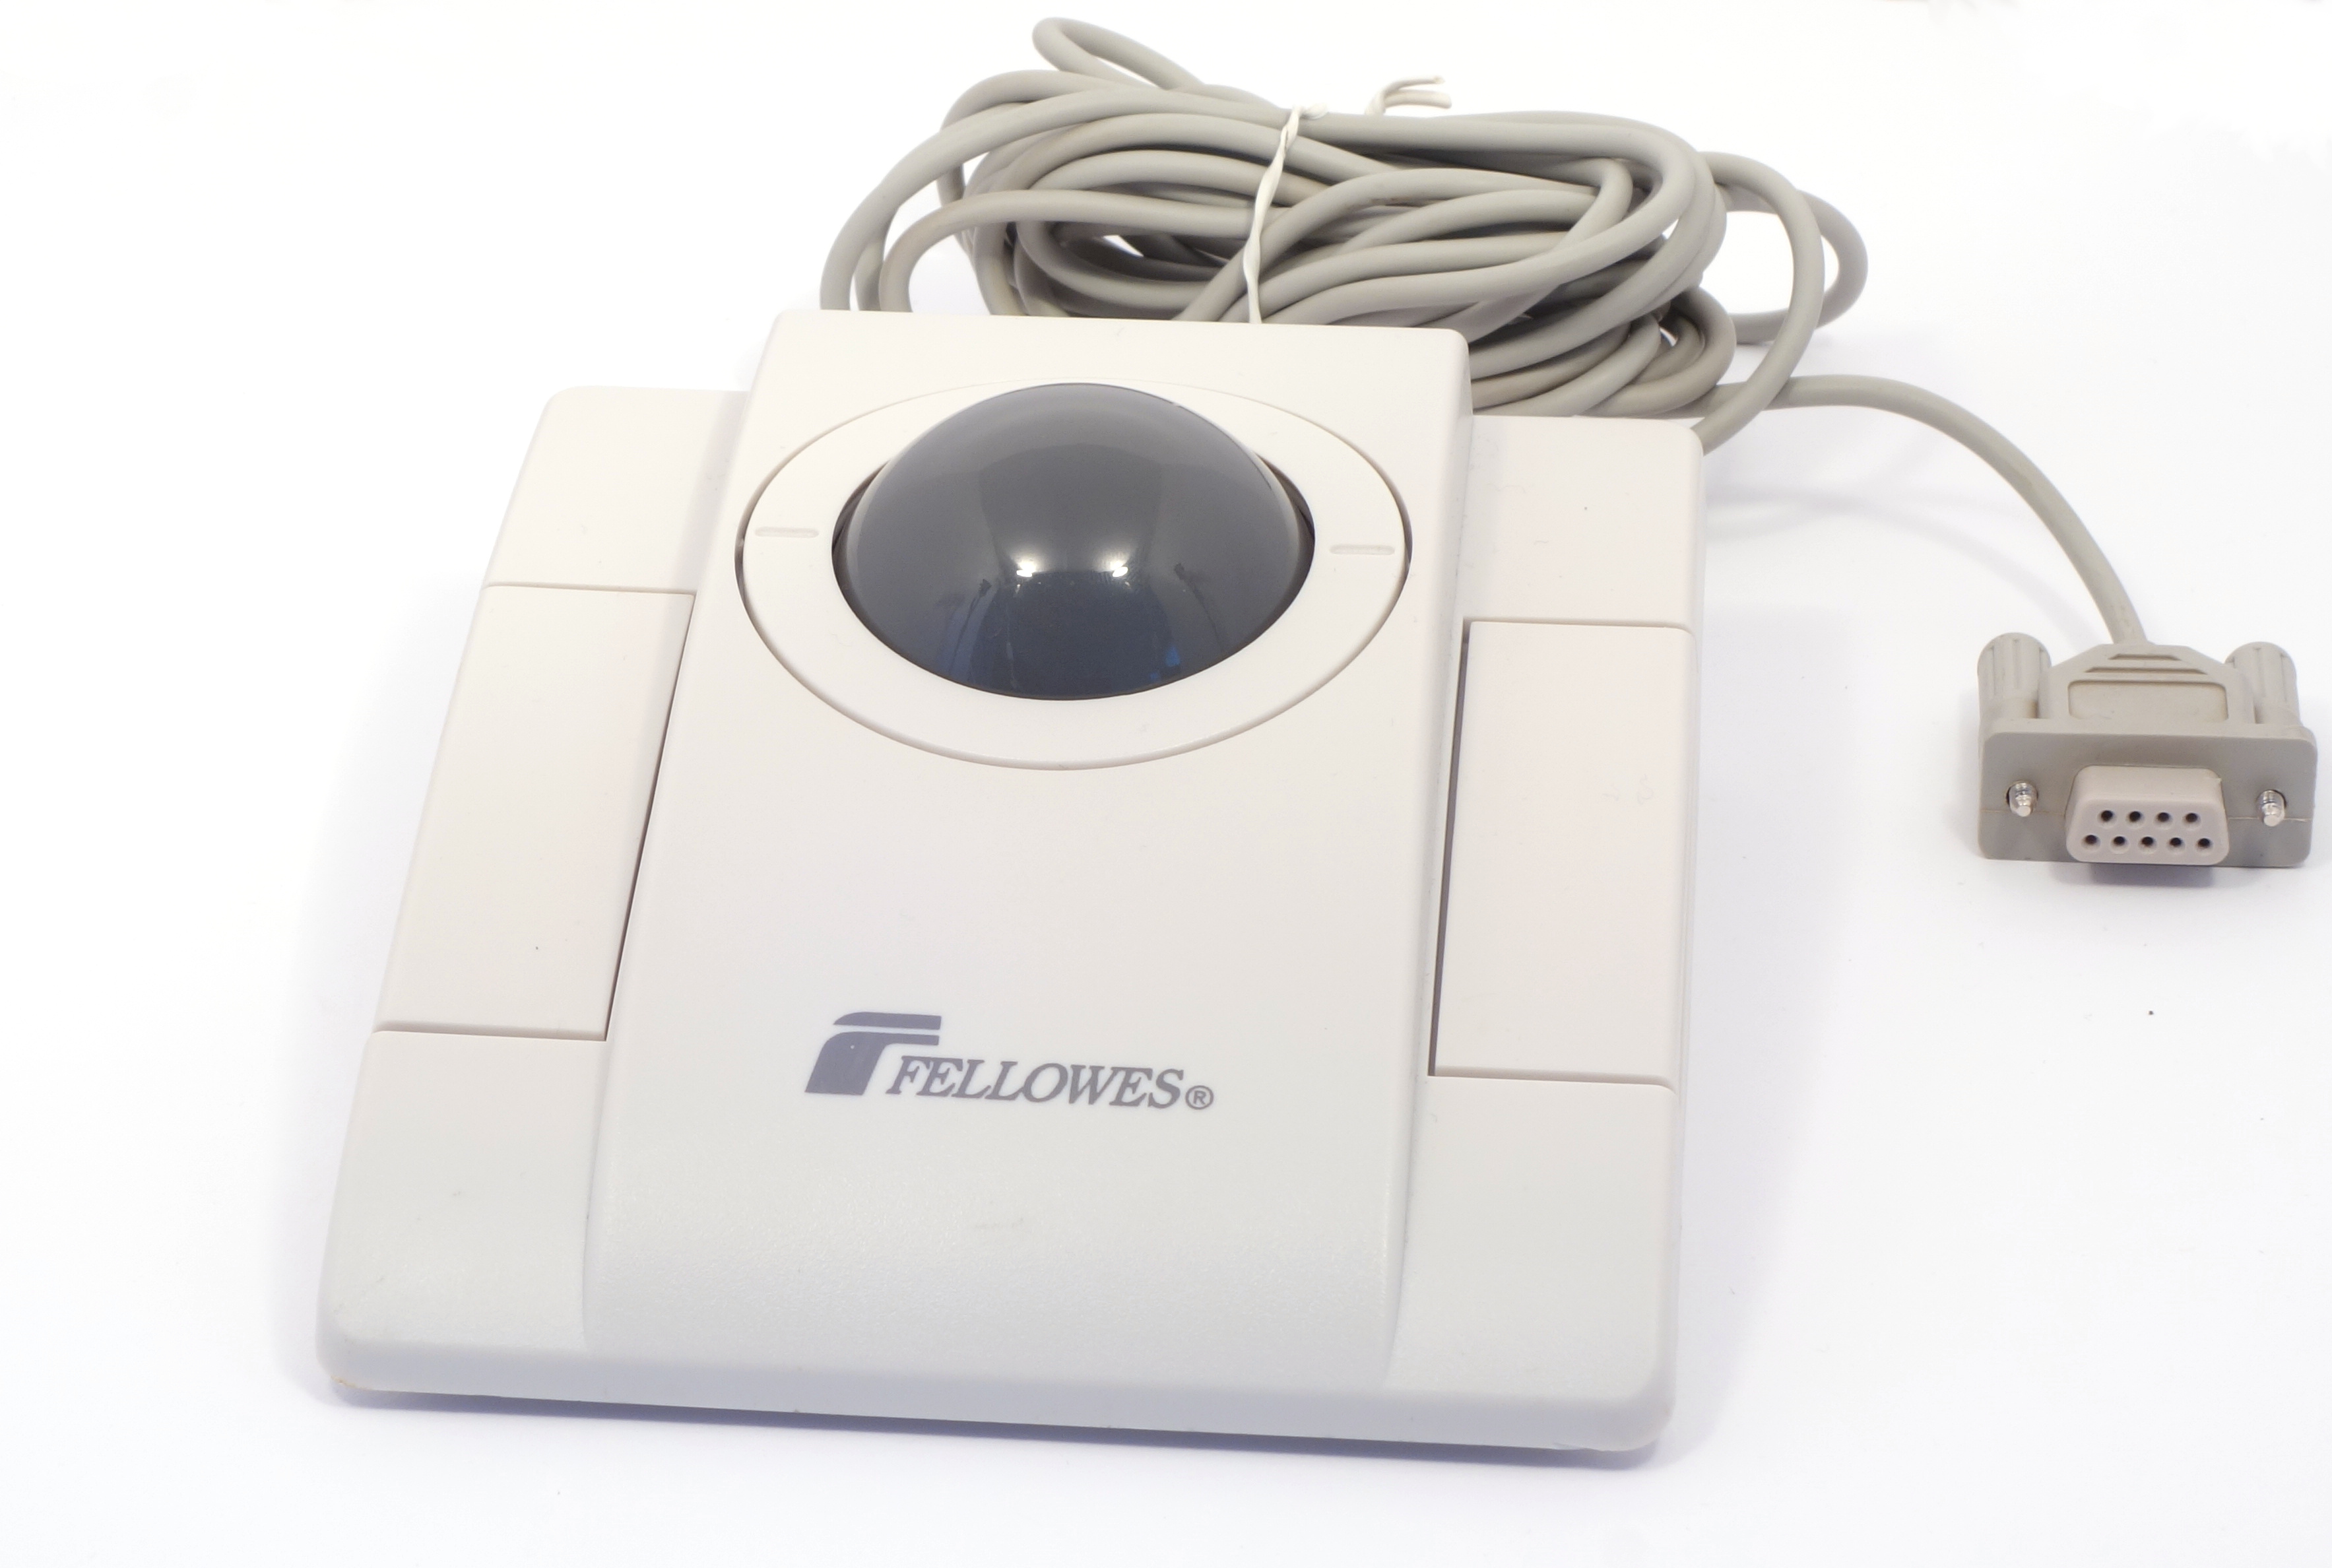
\includegraphics[scale=0.5]{1997_fellowes_trackball/pic_30.jpg}
    \caption{Fellowes Trackball}
    \label{fig:FellowesTrackballPic}
\end{figure}

This trackball has a symmetrical design suitable for both right and left handers (figure \ref{fig:FellowesTrackballTopBottom}).

\begin{figure}[h]
    \centering
    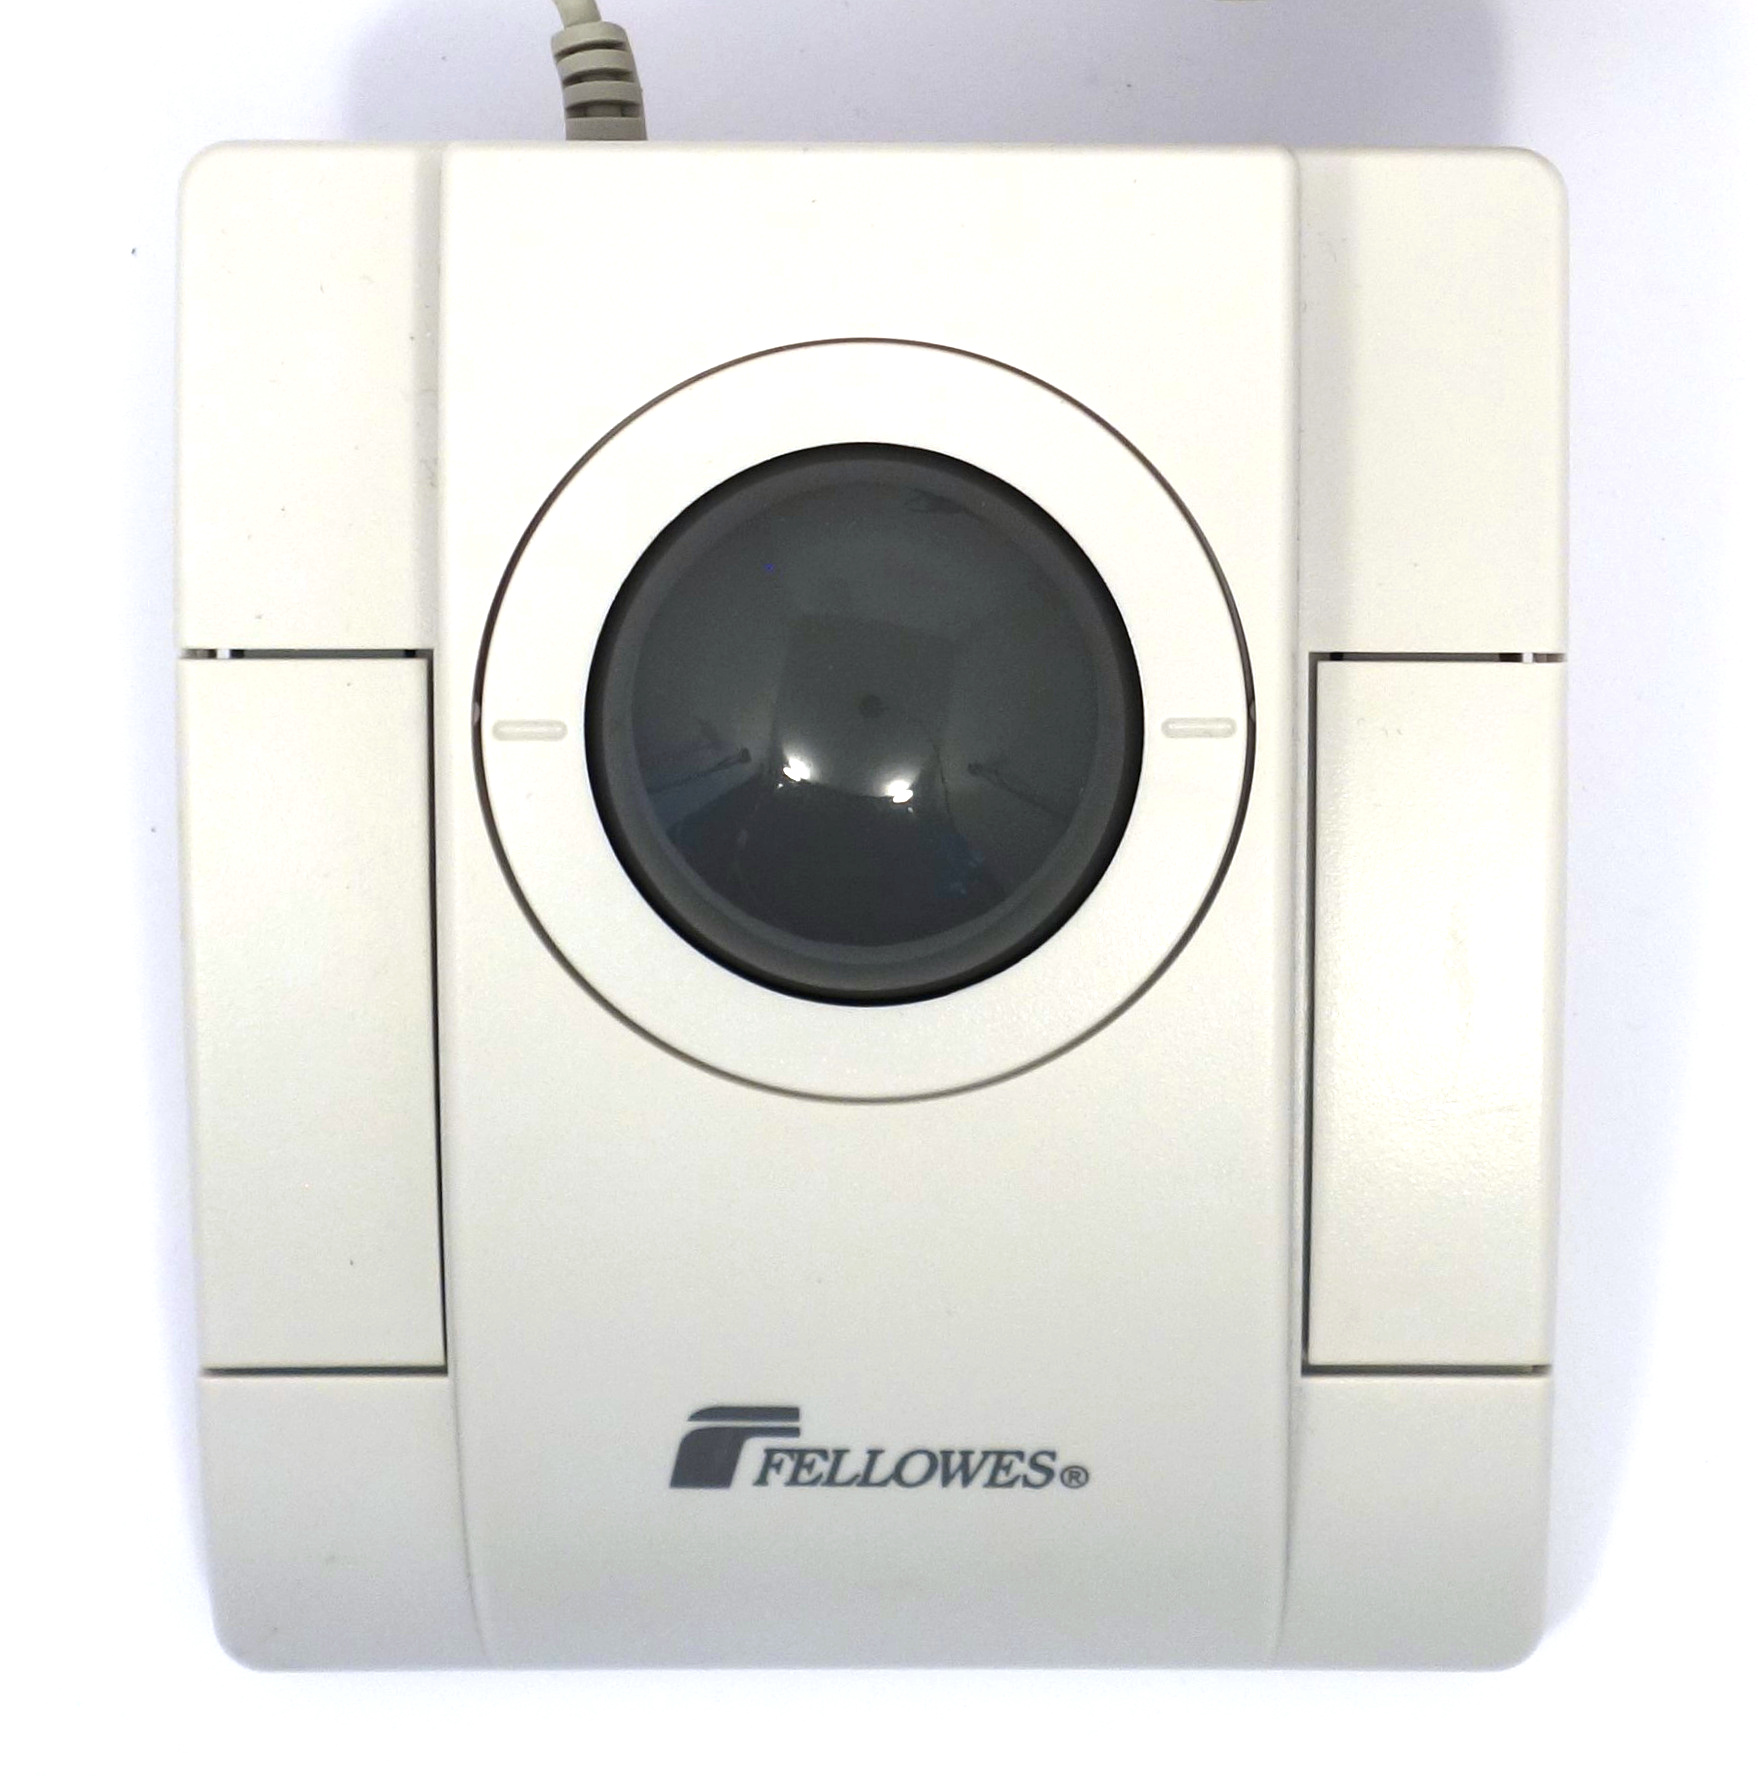
\includegraphics[scale=0.45]{1997_fellowes_trackball/top_60.jpg}
    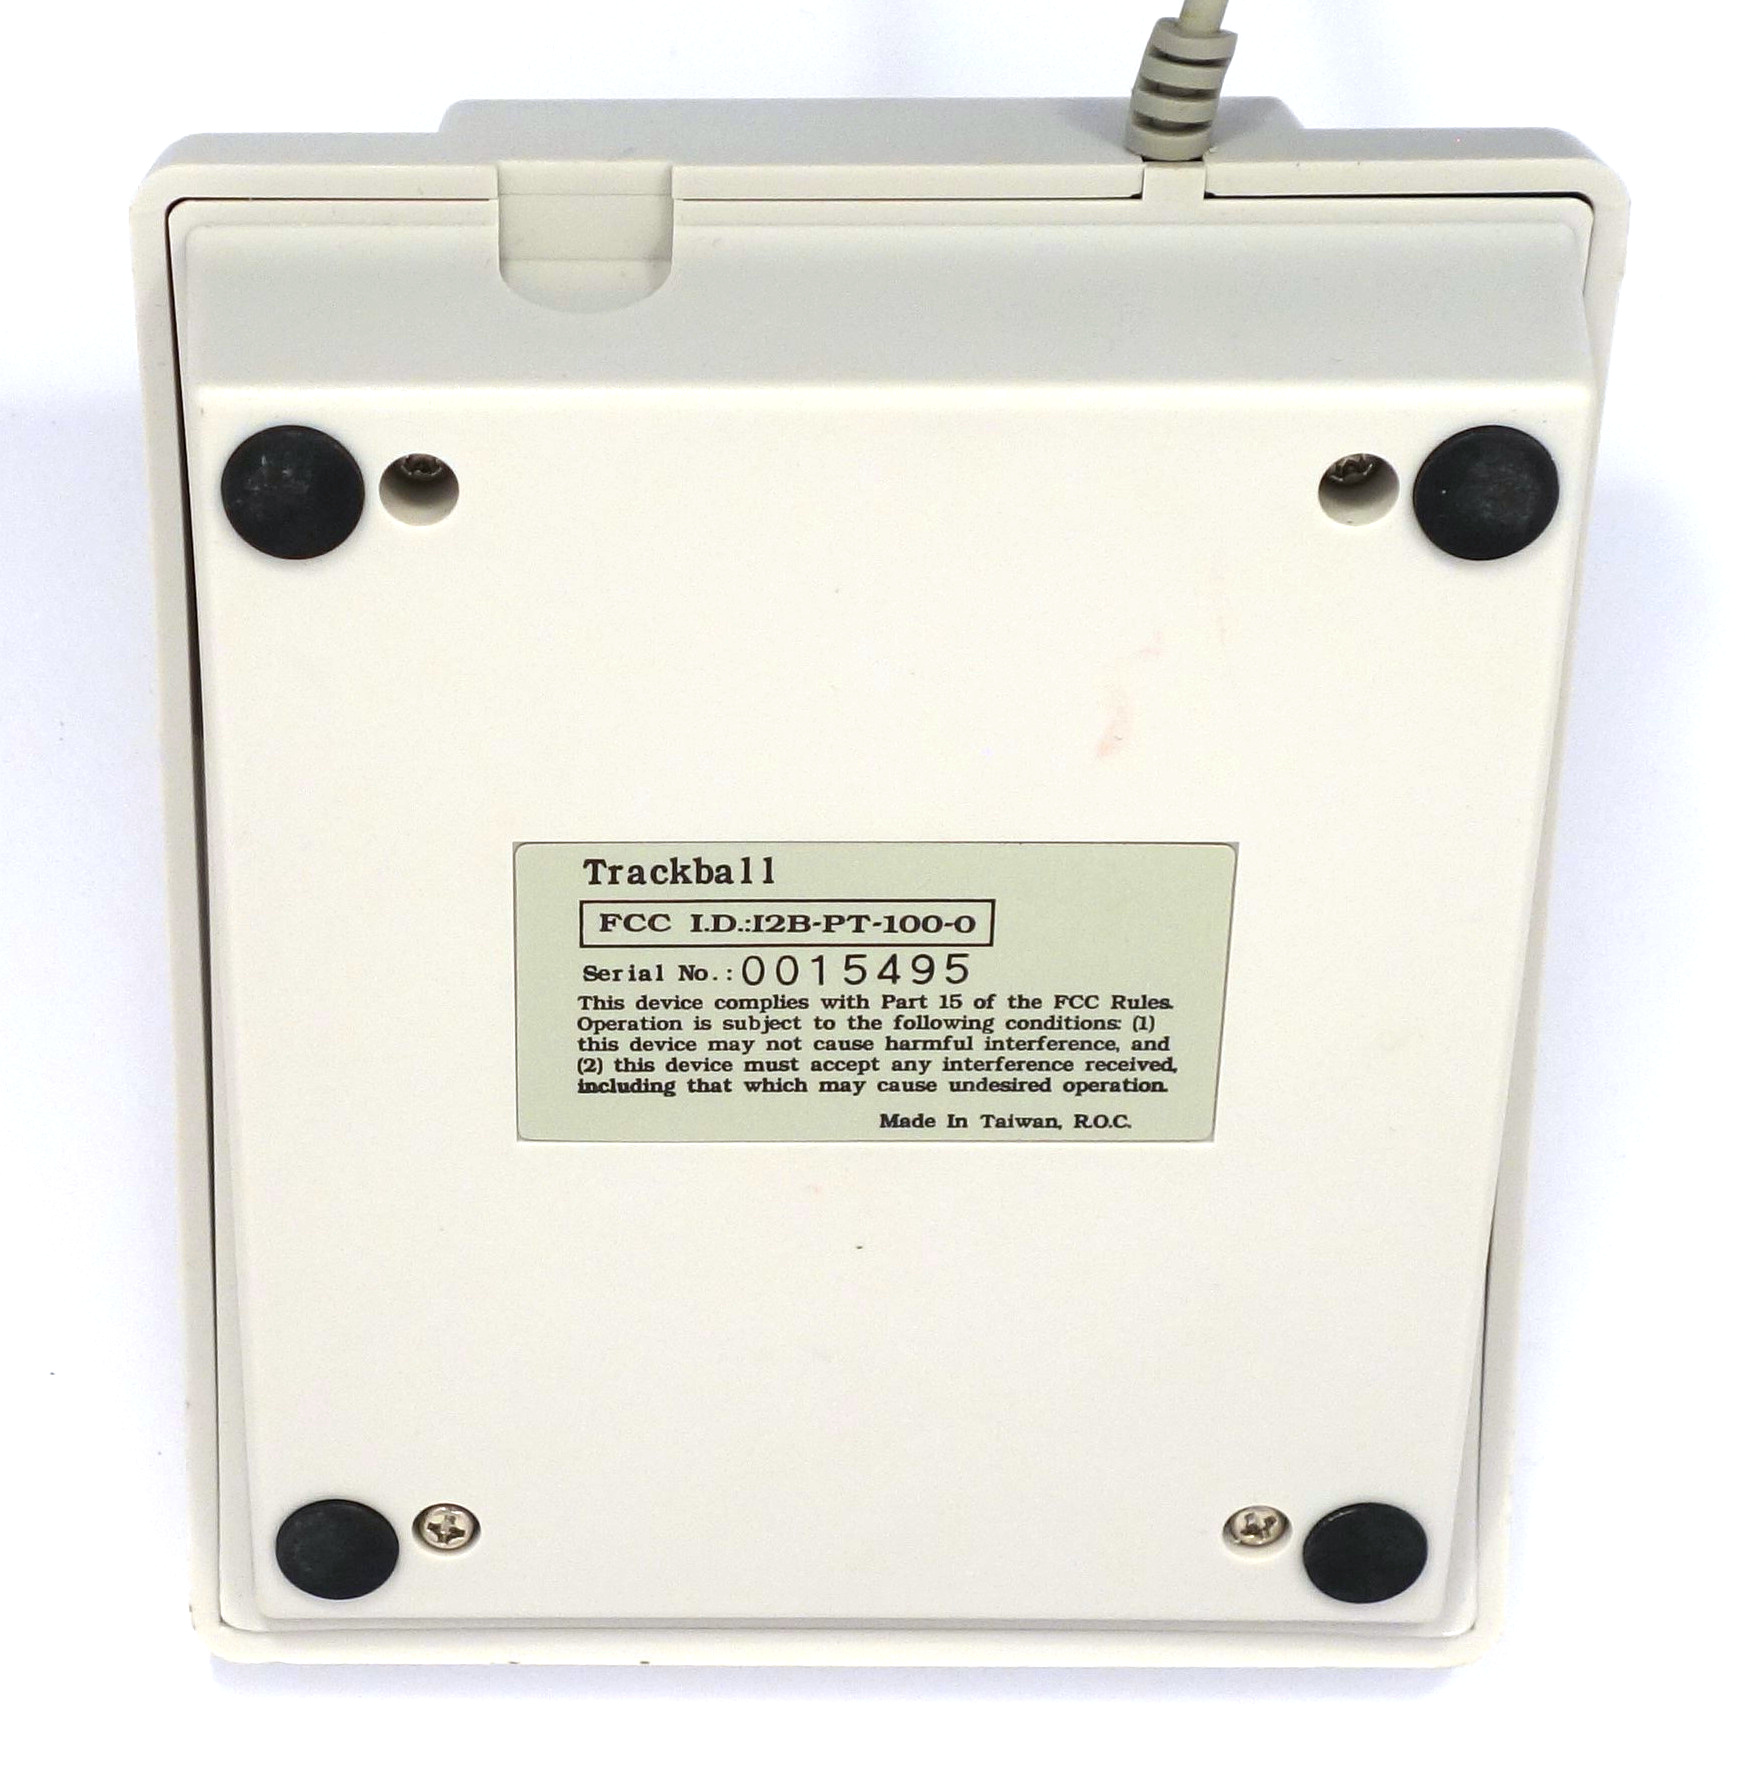
\includegraphics[scale=0.45]{1997_fellowes_trackball/bottom_60.jpg}
    \caption{Fellowes Trackball, top and bottom views}
    \label{fig:FellowesTrackballTopBottom}
\end{figure}

The trackball is large enough (figure \ref{fig:FellowesTrackballSize}); the description in the manufacturer's catalog mentions the precision control achieved by the large diameter ball, as well as the easy removal of the ball for cleaning \cite{advertising}.

\begin{figure}[h]
    \centering
    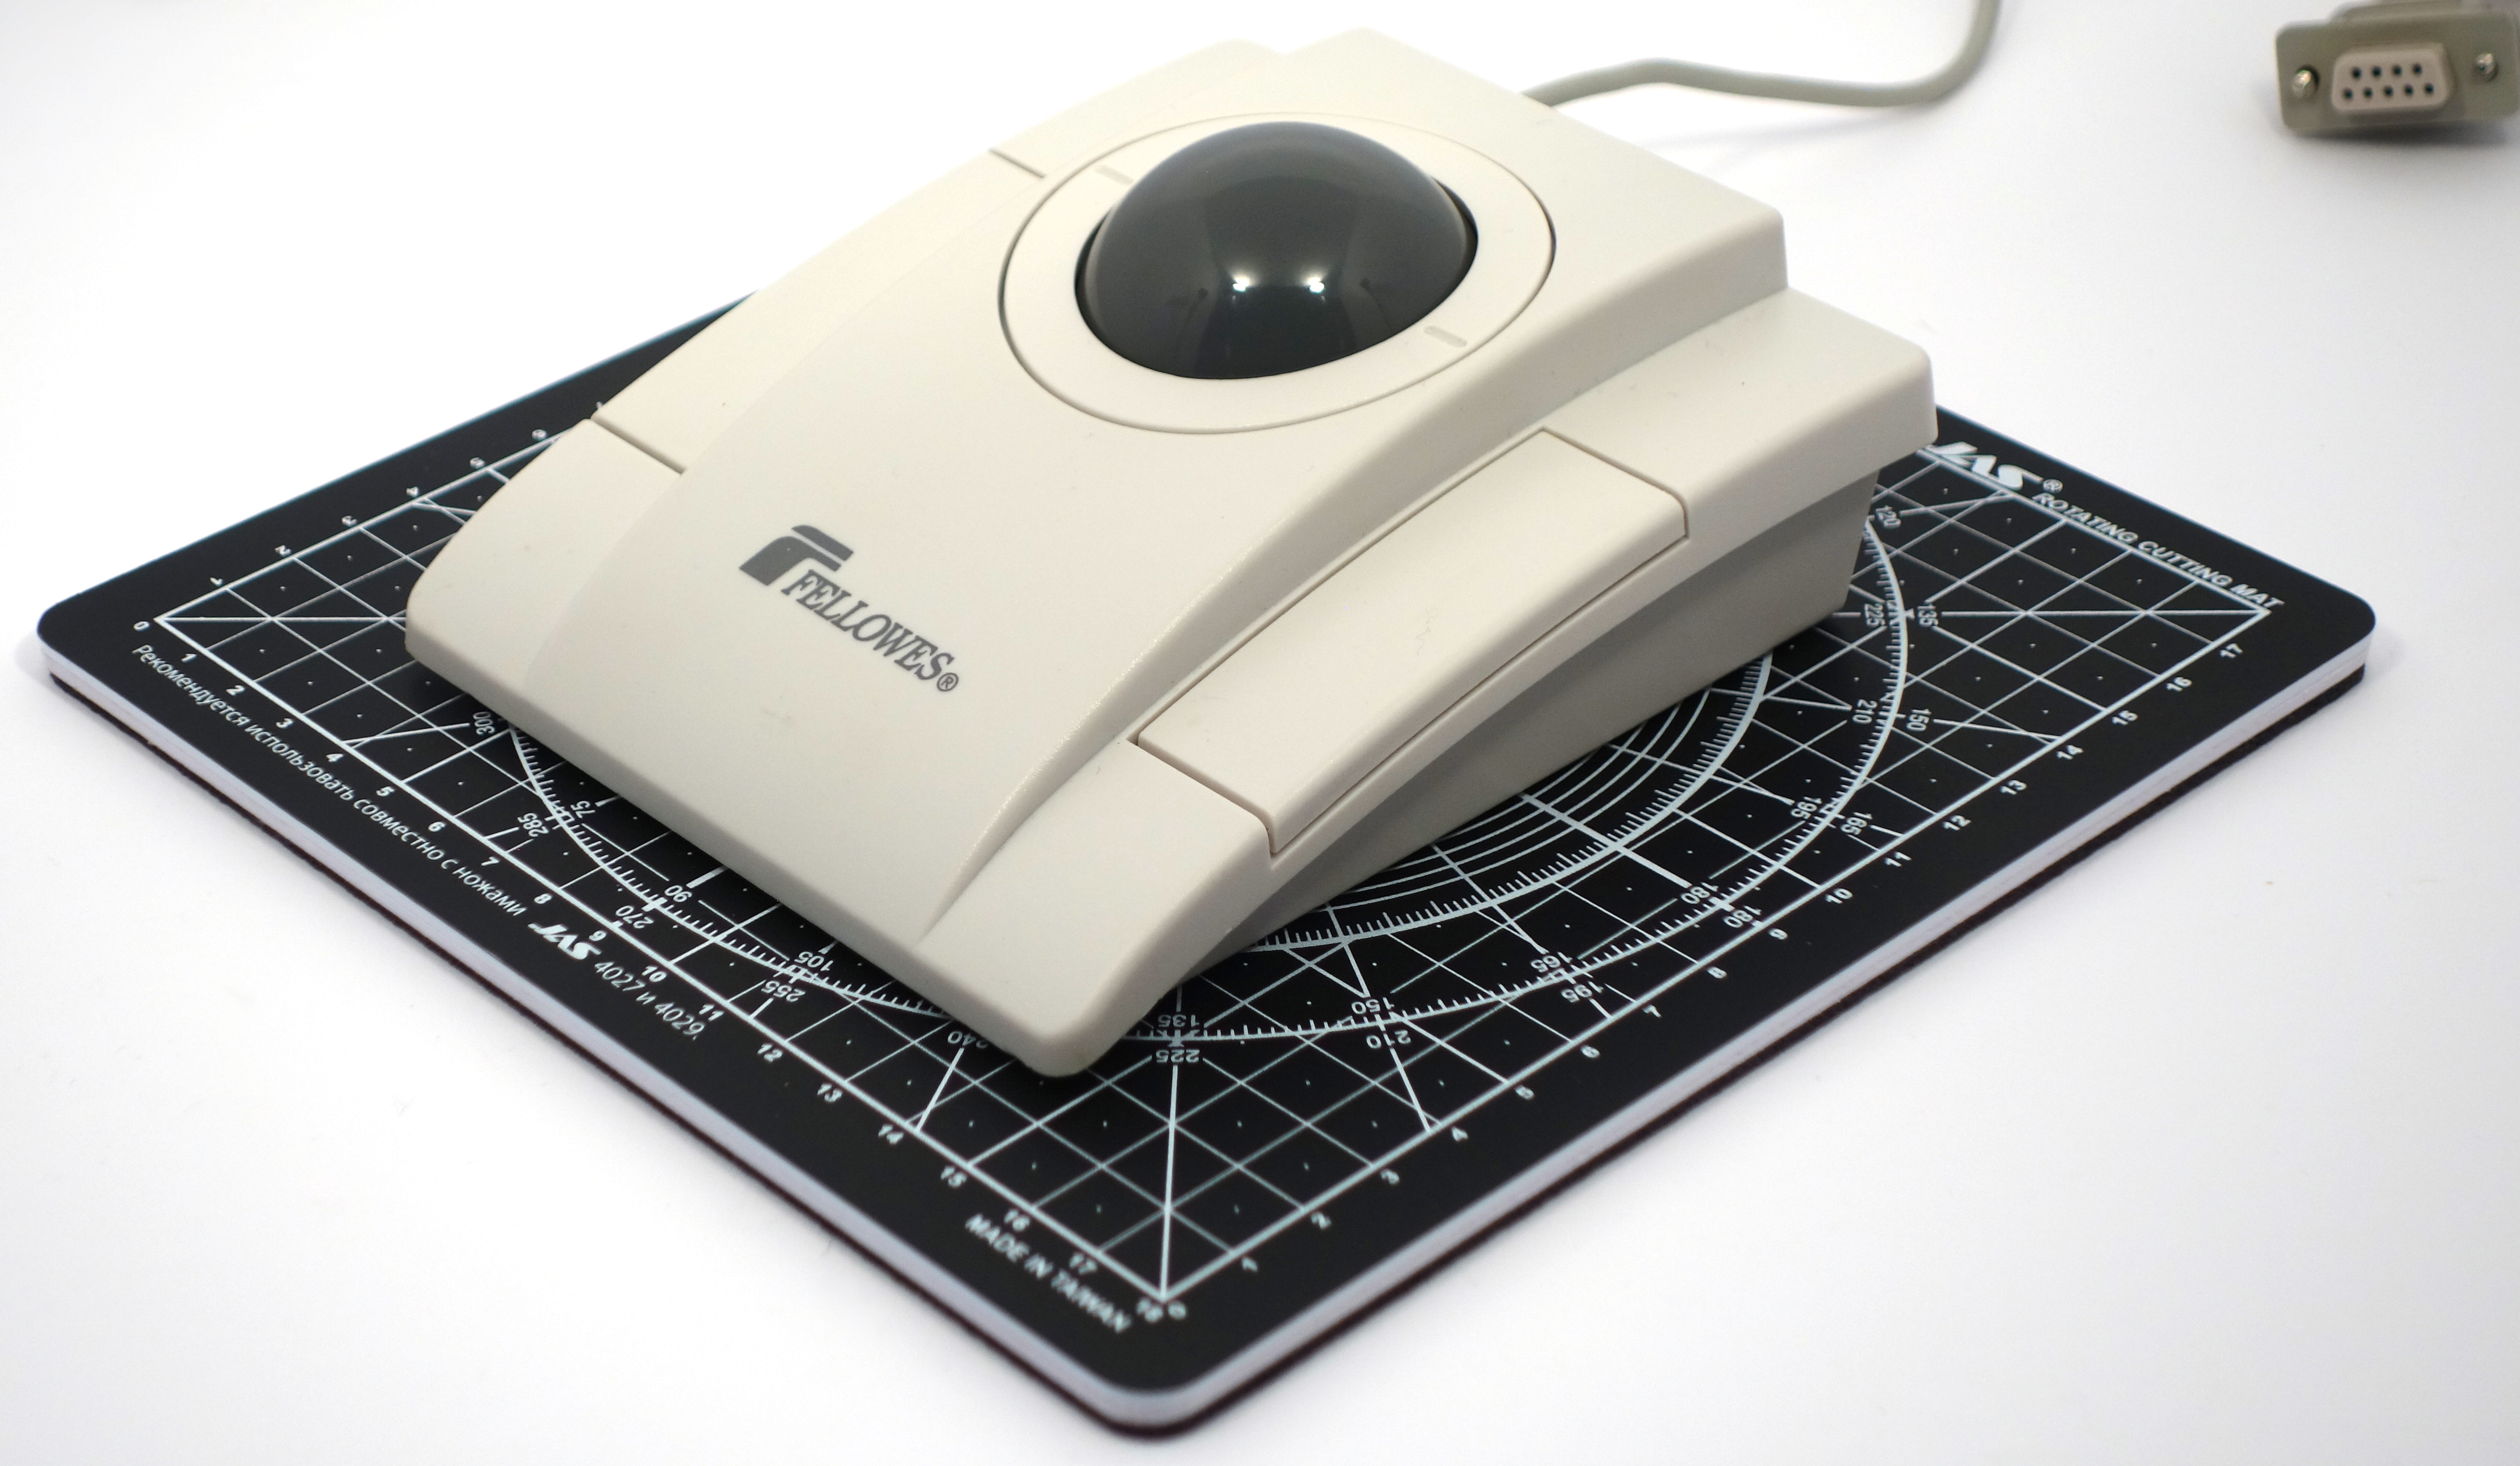
\includegraphics[scale=0.3]{1997_fellowes_trackball/size_30.jpg}
    \caption{Fellowes Trackball on a graduated pad with a grid step of 1~cm}
    \label{fig:FellowesTrackballSize}
\end{figure}

When using a trackball, only the hand and finger movements are used for cursor movement operations. Therefore, the user does not need to move the shoulder and forearm, while the same mouse operations require the use of almost the entire arm. Therefore, the trackball is often recommended for users experiencing temporary or permanent problems associated with the shoulder girdle or wrist.

\begin{figure}[h]
    \centering
    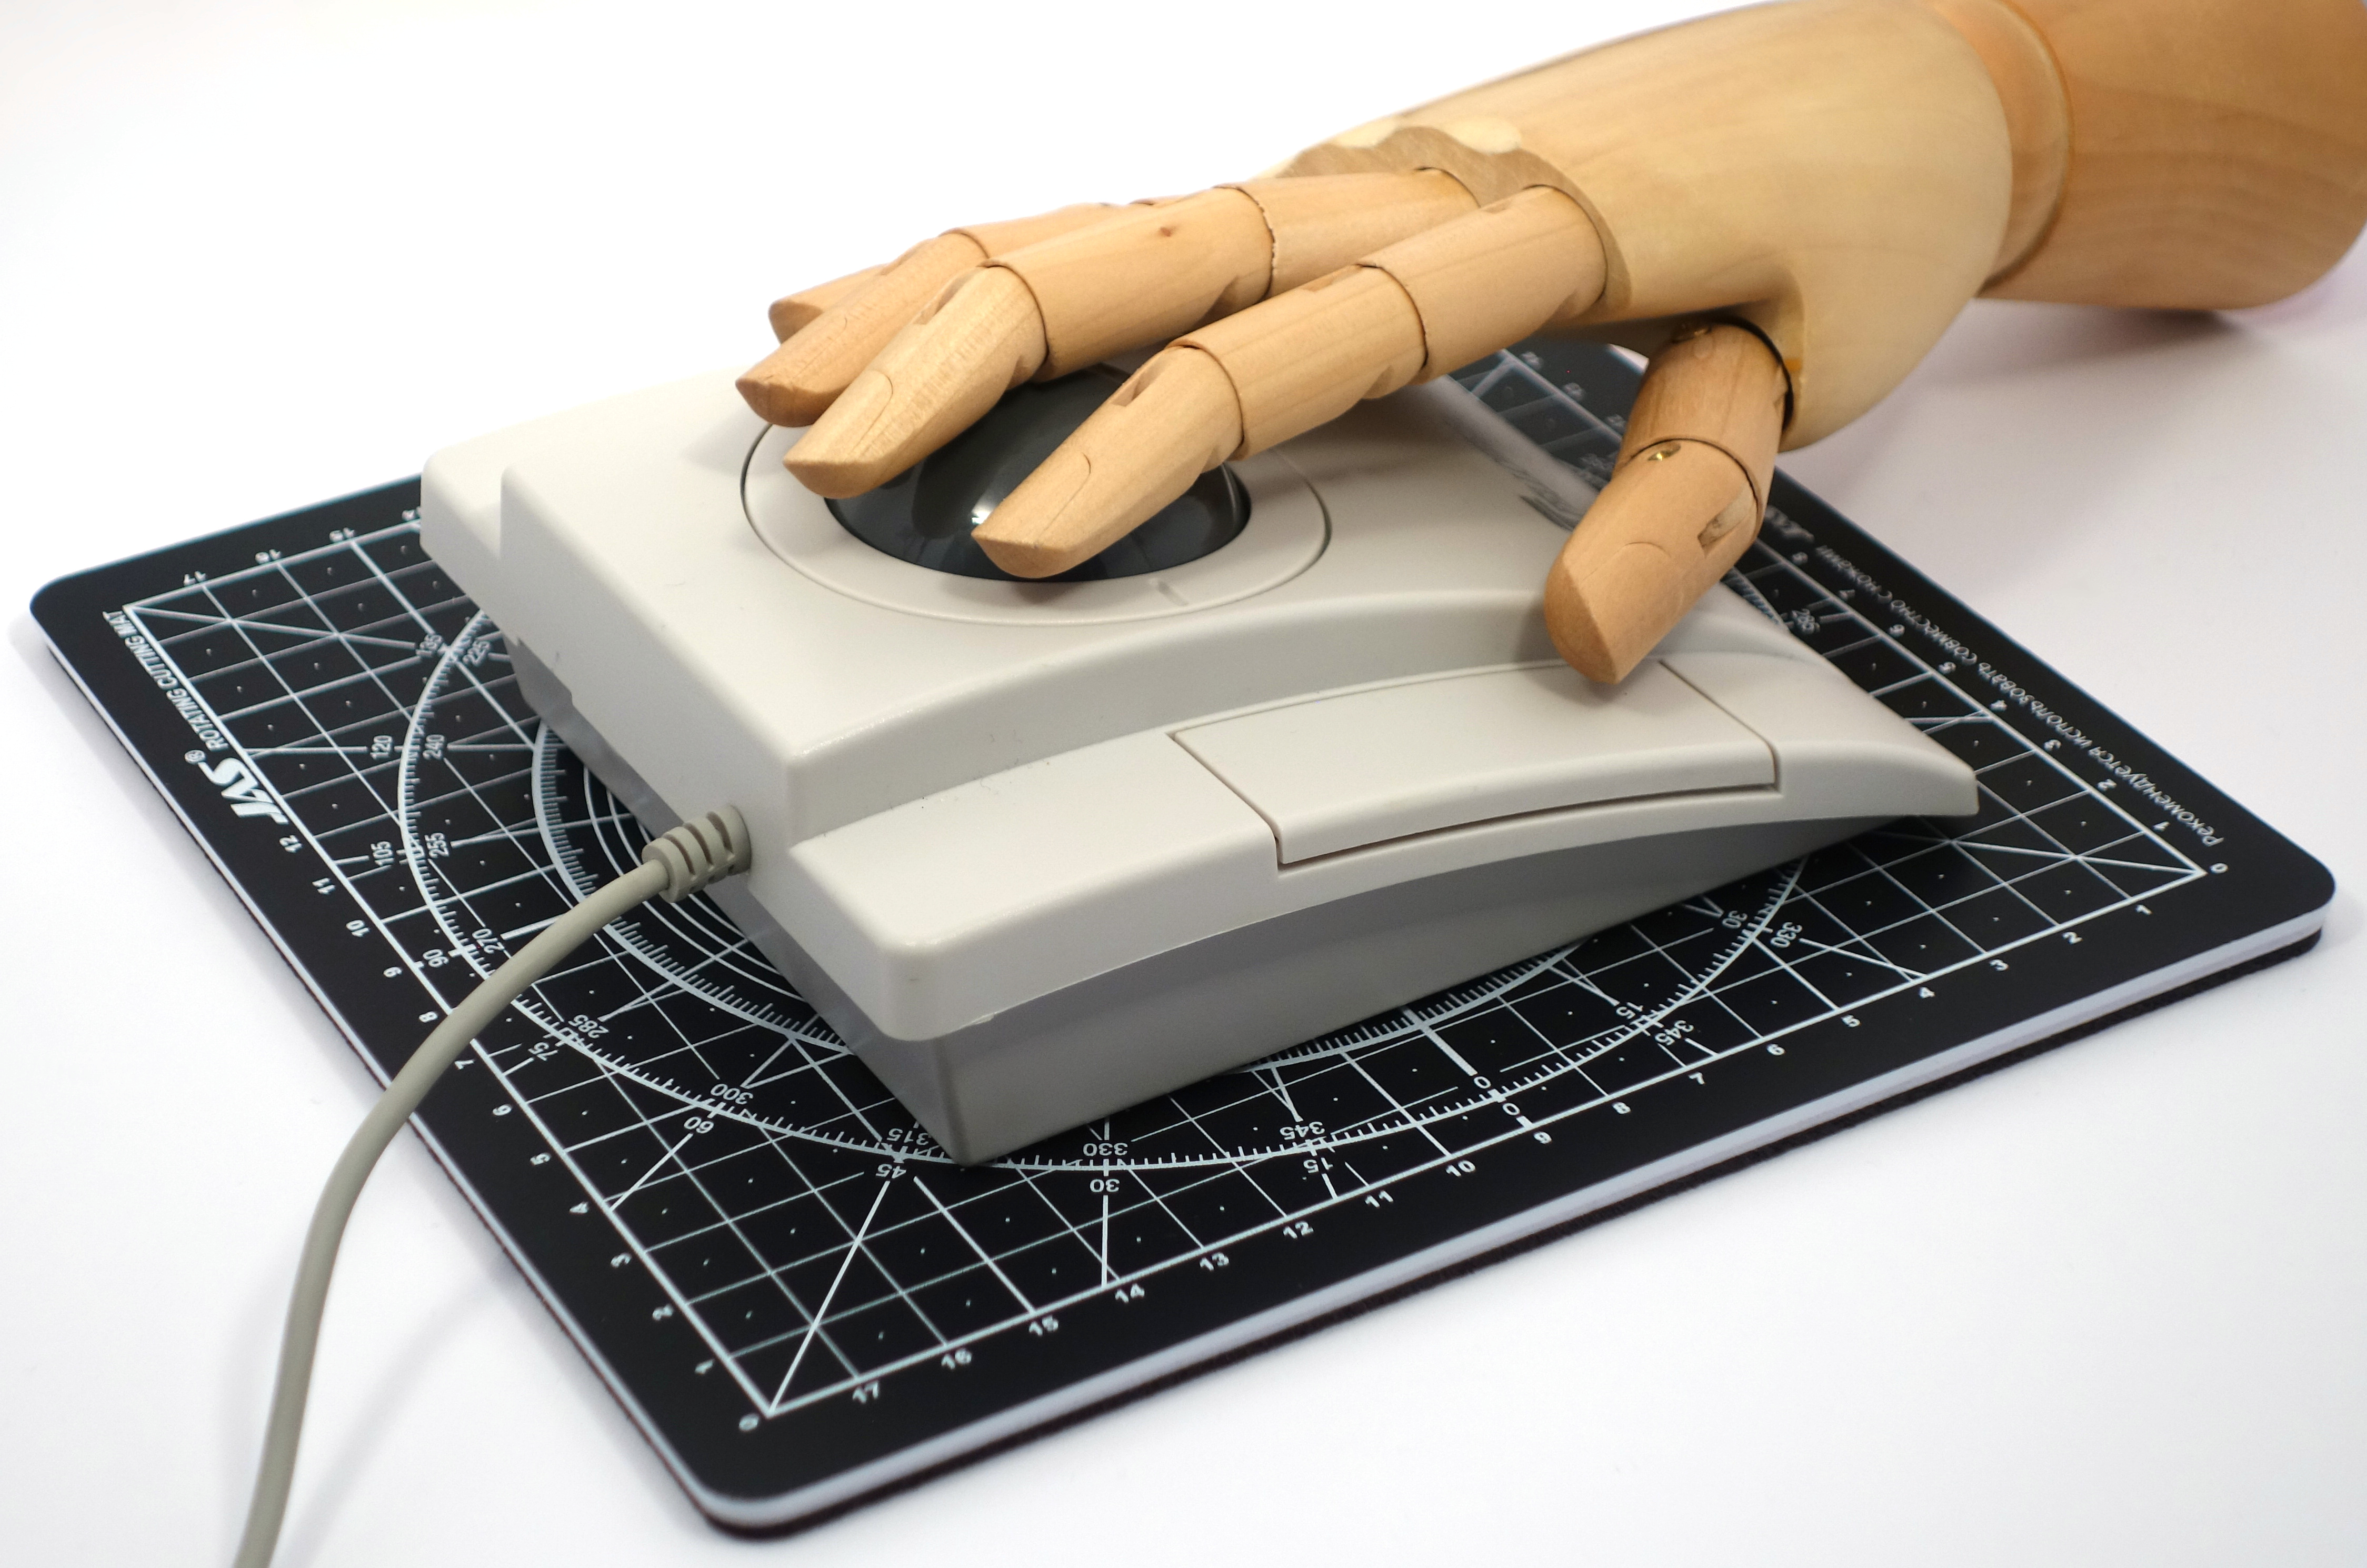
\includegraphics[scale=0.3]{1997_fellowes_trackball/hand_30.jpg}
    \caption{Fellowes Trackball with a human hand model}
    \label{fig:FellowesTrackballHand}
\end{figure}

In terms of ergonomics, we can note the convenient shape of the body and large buttons, but the location of the buttons cannot be called optimal (figure \ref{fig:FellowesTrackballHand}). Using only two buttons symmetrically on the sides of the device looks aesthetically pleasing, but it forces users to spread their fingers as wide as possible -- especially when both buttons need to be pressed at the same time, which could be used to emulate a missing third button or to scroll text by rotating the ball.

\begin{figure}[h]
    \centering
    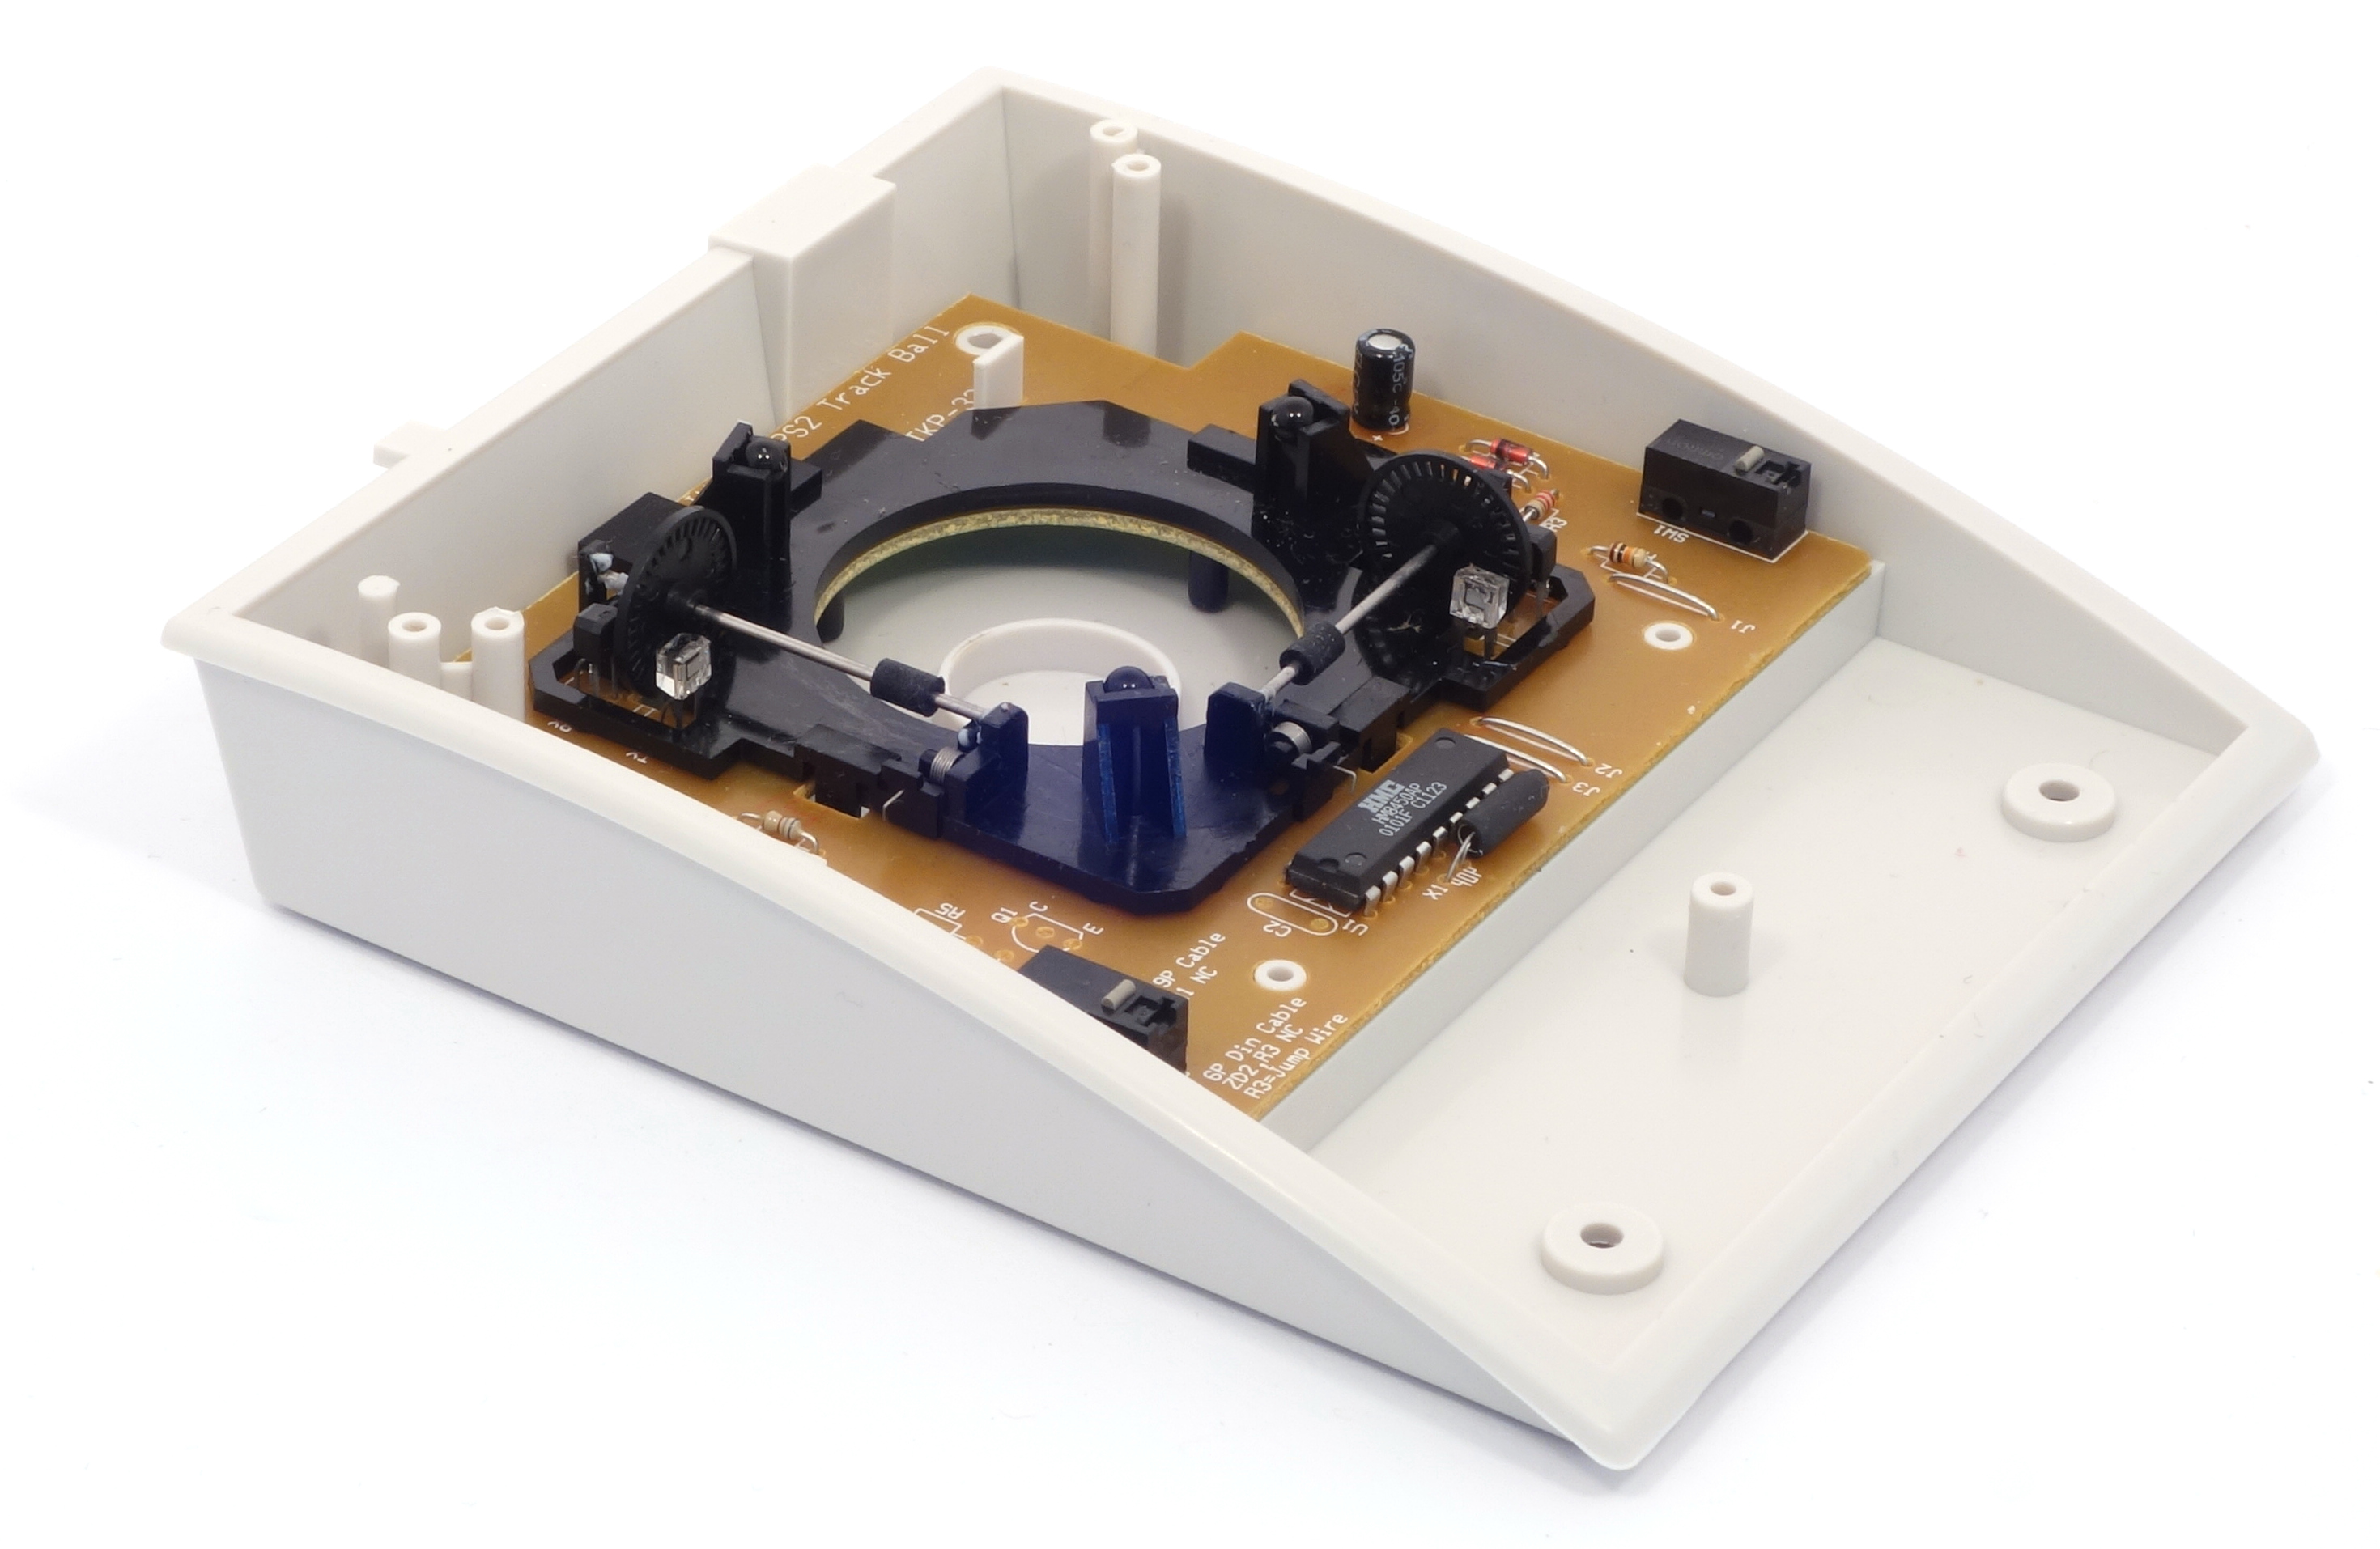
\includegraphics[scale=0.7]{1997_fellowes_trackball/inside_60.jpg}
    \caption{Fellowes Trackball disassembled}
    \label{fig:FellowesTrackballInside}
\end{figure}

Trackball internals are shown on figure \ref{fig:FellowesTrackballInside}. As you can see, it follows the traditional opto-mechanical scheme. In addition to symmetrical design, equally convenient for both the left and right hands, the manufacturer’s advertising focuses on high -quality large area buttons. In terms of compatibility, Windows support is stated from the version 3.1 \cite{advertising}.

\begin{thebibliography}{9}
\bibitem{advertising} Fellowes on-line catalog \url{https://docs.rs-online.com/046b/0900766b8024b417.pdf}
\end{thebibliography}
\end{document}
